% ============================================================================
%  OLK — Open Library Kashmir
%  Developer & Team Kickoff — Technical + Product Overview (~48 min)
%  --------------------------------------------------------------------------
%  Compile with:  pdflatex first_develper.tex   (run twice for numbering)
%  or:            latexmk -pdf first_develper.tex
%  Screenshots in ./screenshots/ are real captures of the running app against
%  a seeded local Docker/Supabase instance — no mockups.
% ============================================================================
\documentclass[aspectratio=169,11pt]{beamer}

\usetheme{metropolis}

% ---------------------------------------------------------------------------
% Brand palette — matches Guide/main.tex and the app's own Tailwind tokens
% ---------------------------------------------------------------------------
\usepackage{xcolor}
\definecolor{olkSlate}{HTML}{0F172A}
\definecolor{olkSlateLight}{HTML}{1E293B}
\definecolor{olkSlateMuted}{HTML}{334155}
\definecolor{olkTeal}{HTML}{14B8A6}
\definecolor{olkTealDark}{HTML}{0D9488}
\definecolor{olkTealLight}{HTML}{2DD4BF}
\definecolor{olkAmber}{HTML}{B45309}
\definecolor{olkGray}{HTML}{64748B}

\setbeamercolor{background canvas}{bg=white}
\setbeamercolor{normal text}{fg=olkSlate}
\setbeamercolor{alerted text}{fg=olkTealDark}
\setbeamercolor{example text}{fg=olkTealDark}
\setbeamercolor{palette primary}{bg=olkSlate,fg=white}
\setbeamercolor{title separator}{fg=olkTeal}
\setbeamercolor{progress bar}{fg=olkTeal,bg=olkSlate!15}
\setbeamercolor{frametitle}{bg=olkSlate,fg=white}
\setbeamercolor{block title}{bg=olkSlate,fg=white}
\setbeamercolor{block body}{bg=olkTeal!8,fg=olkSlate}
\setbeamercolor{block title alerted}{bg=olkAmber,fg=white}
\setbeamercolor{block body alerted}{bg=olkAmber!10,fg=olkSlate}
\setbeamercolor{item}{fg=olkTealDark}
\setbeamercolor{itemize item}{fg=olkTealDark}
\setbeamercolor{itemize subitem}{fg=olkTeal}
\setbeamercolor{section in toc}{fg=olkSlate}
\setbeamercolor{footline}{fg=olkGray}

\metroset{block=fill,progressbar=frametitle,numbering=fraction,sectionpage=progressbar}

% ---------------------------------------------------------------------------
% Diagrams, tables, code, images
% ---------------------------------------------------------------------------
\usepackage{tikz}
\usetikzlibrary{calc,arrows.meta,positioning,fit,backgrounds,shadows.blur}
\usepackage{booktabs}
\usepackage{array}
\usepackage{listings}
\usepackage{graphicx}
\graphicspath{{screenshots/}}

\lstdefinestyle{olkcode}{
  backgroundcolor=\color{olkSlate},
  basicstyle=\ttfamily\scriptsize\color{white},
  breaklines=true,
  columns=fullflexible,
  frame=single,
  framerule=0pt,
  rulecolor=\color{olkSlate},
  framesep=6pt,
  xleftmargin=4pt,
  keywordstyle=\color{olkTealLight}\bfseries,
  commentstyle=\color{olkTealLight}\itshape,
  stringstyle=\color{olkTealLight},
}
\lstset{style=olkcode}

\newcommand{\code}[1]{\textcolor{olkTealDark}{\texttt{#1}}}
\newcommand{\pathname}[1]{\textcolor{olkSlateLight}{\texttt{#1}}}

% Consistent framed screenshot helper — a thin slate border so every capture
% reads as "real app in a window", not a loose image floating on a slide.
\newcommand{\shot}[2][width=\linewidth]{%
  \fbox{\includegraphics[#1]{#2}}%
}

\title{OLK --- Open Library Kashmir}
\subtitle{A Technical \& Product Deep Dive}
\author{OLK Engineering}
\date{\today}

\begin{document}

% ============================================================================
\begin{frame}
  \titlepage
\end{frame}

% ----------------------------------------------------------------------------
\begin{frame}{Agenda --- roughly 48 minutes}
  \small
  \begin{tabular}{@{}p{8cm}r@{}}
    \textbf{Why OLK exists} --- the real story, and the constraint that shapes everything & 6 min \\[2pt]
    \textbf{A live tour of the platform} --- real screens, for everyone in the room & 12 min \\[2pt]
    \textbf{Tech stack at a glance} --- what it's built with, and why & 4 min \\[2pt]
    \textbf{Under the hood} --- architecture, database, security, GPS, deploy & 16 min \\[2pt]
    \textbf{The road ahead} --- mobile, self-hosting, scaling responsibly & 6 min \\[2pt]
    \textbf{Get involved \& discussion} & 4 min \\
  \end{tabular}
  \vspace{8pt}
  \begin{alertblock}{One honest note before we start}
    \small This deck is a companion to the full technical manual at \code{Guide/main.pdf} --- every claim here traces back to a chapter, a migration, or a line of code there. Every screenshot in this deck is a real capture of the running app, not a mockup.
  \end{alertblock}
\end{frame}

% ============================================================================
\section{Why OLK Exists}

\begin{frame}{How this actually started}
  OLK didn't begin as software. It began as \textbf{volunteers physically collecting donated books and hand-delivering them to students} across the Kashmir valley.
  \vspace{4pt}
  \begin{itemize}
    \item That model hit a real wall: never enough volunteers, never enough donors, and a distribution network too thin to reach the students who needed it.
    \item The fix wasn't more volunteers --- it was removing the middle layer entirely.
  \end{itemize}
  \vfill
  \begin{block}{The pivot}
    Instead of a warehouse in the middle, put the two people directly in touch: the one with a book, and the one who wants to read it. That is the entire product.
  \end{block}
\end{frame}

\begin{frame}{What is OLK, today?}
  \textbf{Open Library Kashmir} is a community book-sharing platform for readers in the Kashmir valley.
  \begin{itemize}
    \item Someone with books on a shelf lists them --- to \alert{lend} (they get it back) or \alert{donate} (they don't).
    \item Someone who wants to read finds them by browsing \alert{nearby} listings and sends a request.
    \item The two arrange an in-person handover.
  \end{itemize}
  \vfill
  \begin{block}{No shipping. No warehouses. No payments.}
    The entire transaction is a conversation between two neighbours and a walk to a bus stop.
  \end{block}
\end{frame}

\begin{frame}{The one design decision that explains everything else}
  \textbf{Everything happens in person, within walking or short-commute distance.}
  \vspace{4pt}

  That is not a missing feature --- it is \emph{the} product decision. It explains:
  \begin{itemize}
    \item why every book and every club carries a latitude/longitude \emph{and} a plain-language area name;
    \item why the database has a distance function instead of a shipping-address field;
    \item why there is no payment table anywhere in the schema;
    \item why \alert{trust} --- ratings, warnings, bans, reports --- matters as much as inventory.
  \end{itemize}
\end{frame}

\begin{frame}{Where we are today}
  \begin{columns}[T]
    \column{0.5\textwidth}
    \textbf{Product}
    \begin{itemize}
      \item Full exchange lifecycle, live
      \item Wishlists, clubs \emph{and now club events}
      \item Admin \& moderation subsystem --- 10 dedicated pages
      \item Regionally real: 29 seeded Kashmir areas across 10 districts, 19 genres
    \end{itemize}
    \column{0.5\textwidth}
    \textbf{Engineering}
    \begin{itemize}
      \item 27 database tables, all RLS-protected
      \item 32 chronological migrations
      \item Local Docker stack mirrors production
      \item A full internal technical manual, chapter per subsystem
    \end{itemize}
  \end{columns}
  \vfill
  \begin{alertblock}{The founder's two goals, in order}
    First: serve real readers in Kashmir, live, on the web. Second: eventually run the platform's own infrastructure --- including the database --- on a physical server \emph{in} Kashmir, not on rented foreign infrastructure.
  \end{alertblock}
\end{frame}

% ============================================================================
\section{A Live Tour of the Platform}

\begin{frame}{This is the actual app}
  \begin{center}
  \shot[width=0.92\linewidth]{landing.png}
  \end{center}
\end{frame}

\begin{frame}{Discover \& share a book}
  \begin{center}
  \shot[width=0.62\linewidth]{browse.png}
  \end{center}
  \vspace{-2pt}
  \footnotesize Browse sorts by real distance, not just recency, and filters by genre, condition, listing type, and area.
\end{frame}

\begin{frame}[fragile]{List a book in seconds --- the ISBN scanner}
  \begin{center}
    \fbox{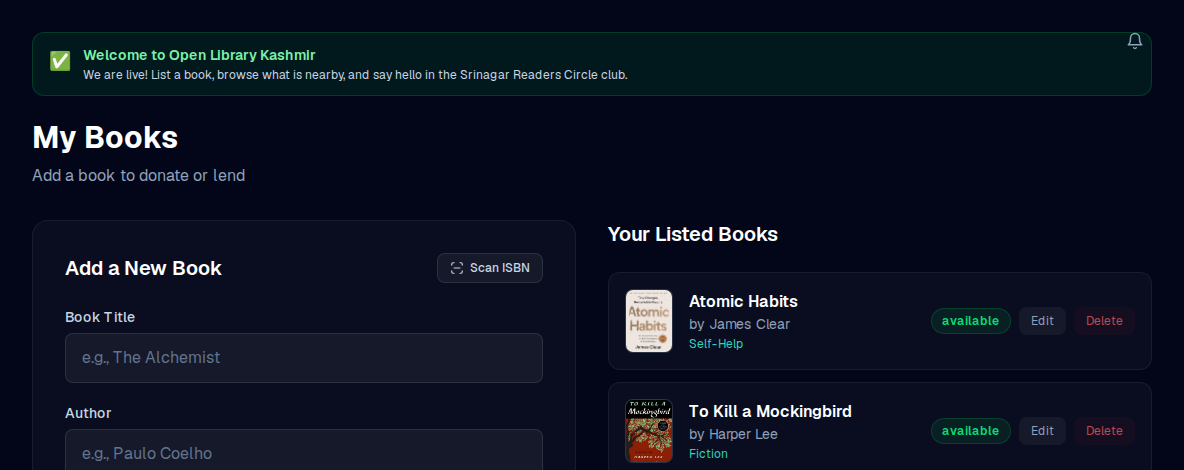
\includegraphics[height=2.6cm]{my-books.png}}\hspace{4pt}%
    \fbox{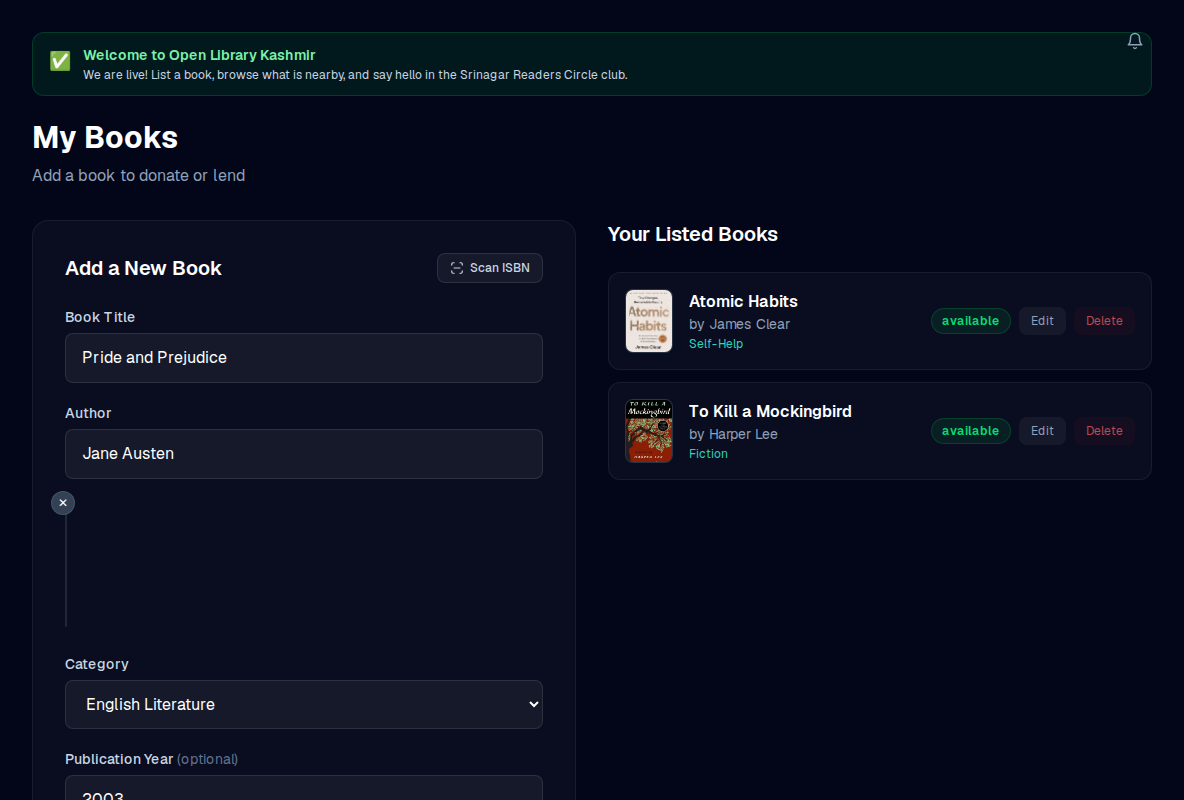
\includegraphics[height=2.6cm]{isbn-autofill.png}}
  \end{center}
  \vspace{4pt}
  \begin{exampleblock}{Point your camera at the barcode}
    \footnotesize Scans the ISBN, looks it up on the free, open Open Library catalogue, and auto-fills title, author, cover image, publication year, description, and even guesses a genre --- \emph{conservatively}: if it isn't confident, it leaves the field blank rather than guessing wrong.
  \end{exampleblock}
\end{frame}

\begin{frame}{From request to handover}
  \begin{center}
  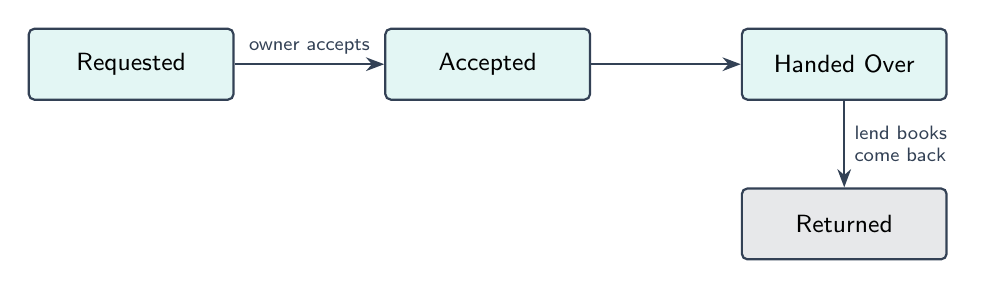
\begin{tikzpicture}[
    st/.style={draw=olkSlateMuted, thick, rounded corners=2pt, fill=olkTeal!12, minimum width=2.6cm, minimum height=0.9cm, font=\sffamily\small, align=center},
    term/.style={st, fill=olkSlate!10},
    arr/.style={-Stealth, thick, olkSlateMuted}
  ]
    \node[st] (pending) {Requested};
    \node[st, right=1.9cm of pending] (accepted) {Accepted};
    \node[st, right=1.9cm of accepted] (handed) {Handed Over};
    \node[term, below=1.1cm of handed] (returned) {Returned};
    \draw[arr] (pending) -- node[above,font=\scriptsize\sffamily]{owner accepts} (accepted);
    \draw[arr] (accepted) -- (handed);
    \draw[arr] (handed) -- node[right,font=\scriptsize\sffamily,align=left]{lend books\\come back} (returned);
  \end{tikzpicture}
  \end{center}
  \vspace{2pt}
  \begin{center}
  \fbox{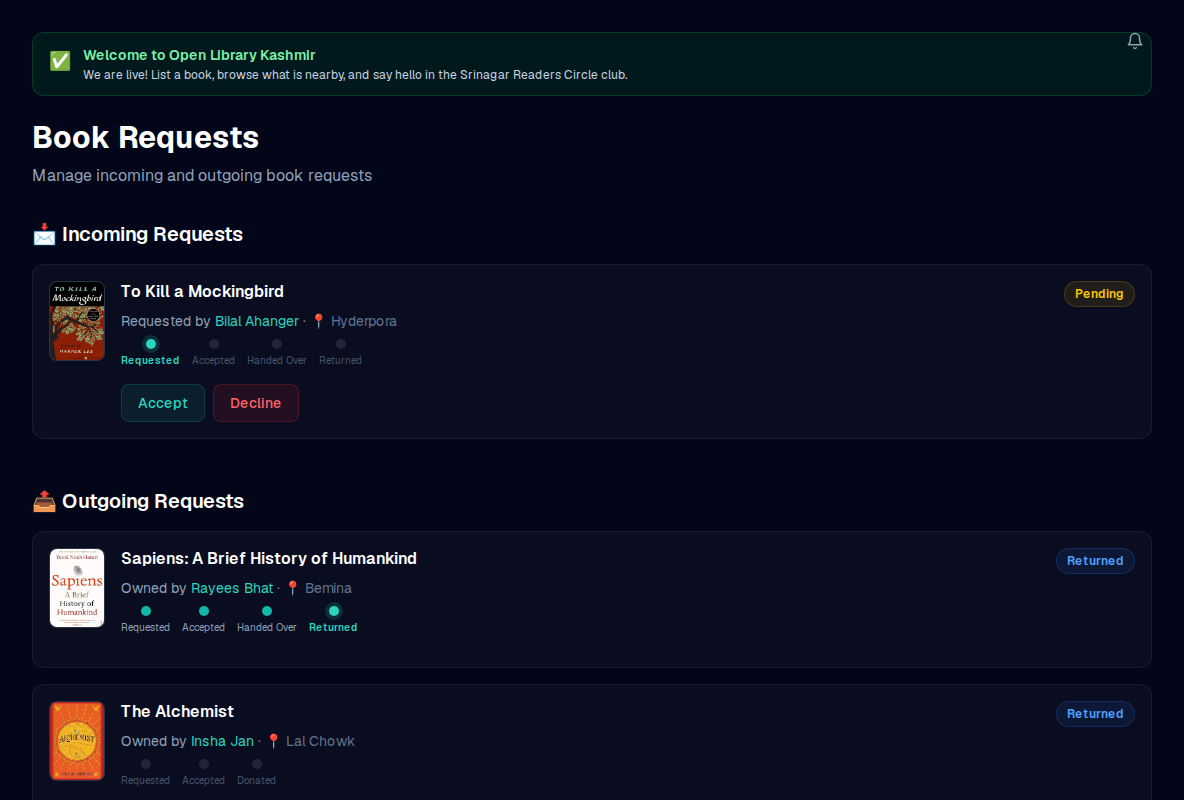
\includegraphics[height=3.0cm]{requests.png}}
  \end{center}
\end{frame}

\begin{frame}{Two ways a book's story ends}
  \begin{columns}[T]
    \column{0.48\textwidth}
    \textbf{Lending}
    \begin{itemize}
      \item Book comes back --- marked \emph{Returned}
      \item Owner keeps it, can lend again
    \end{itemize}
    \column{0.48\textwidth}
    \textbf{Donating}
    \begin{itemize}
      \item ``\textbf{Pass It On}'' when the reader is done
      \item Ownership transfers --- permanently
      \item The new owner can re-list it, and it can never quietly become a private copy again
    \end{itemize}
  \end{columns}
  \vfill
  \begin{block}{One shared counter}
    Every book carries a \code{read\_count} --- incremented on \emph{both} paths, so a donated book that's changed hands five times and a book that's been lent out five times both show up equally as ``reached five readers.''
  \end{block}
\end{frame}

\begin{frame}{Chat, rate, build trust}
  \begin{center}
  \shot[width=0.62\linewidth]{chat.png}
  \end{center}
  \vspace{-2pt}
  \footnotesize Every request gets its own realtime 1:1 chat. After a handover, both sides leave a 1--5 star rating; enough good ratings earns a public ``Trusted Sharer'' badge --- there's no escrow or shipping carrier here, so reputation \emph{is} the safety net.
\end{frame}

\begin{frame}{Can't find a book? Wishlist it.}
  \begin{columns}[T]
    \column{0.55\textwidth}
    \begin{enumerate}
      \item You add \emph{``The Old Man and the Sea''} to your wishlist. Nothing happens yet.
      \item Weeks later, someone --- a total stranger --- lists a copy, typed slightly differently.
      \item The platform notices the match \textbf{automatically} and notifies you.
    \end{enumerate}
    \column{0.4\textwidth}
    \shot{wishlist.png}
  \end{columns}
  \vfill
  \begin{block}{``Smart'' matching, honestly explained}
    It's a fuzzy text-similarity search across \emph{every} user's wishlist, not just yours --- something that needs a deliberate, careful piece of backend engineering to do safely (Part IV).
  \end{block}
\end{frame}

\begin{frame}{Reading clubs --- now with events}
  \begin{center}
    \fbox{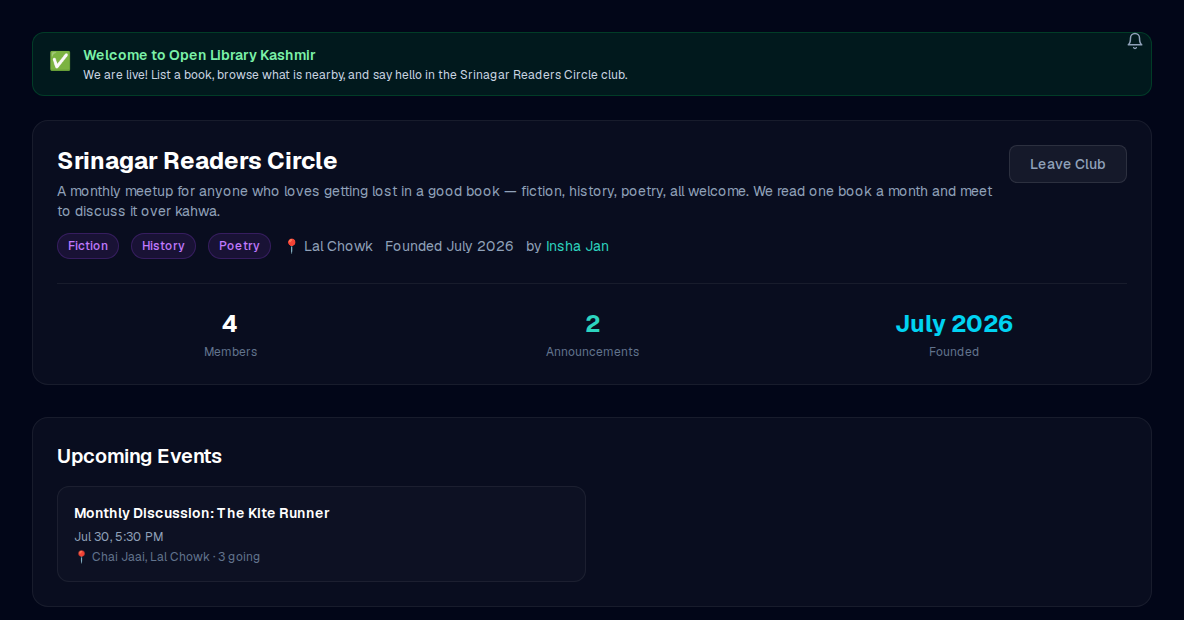
\includegraphics[height=2.3cm]{club-detail.png}}\hspace{4pt}%
    \fbox{
\includegraphics[height=2.3cm]{event-detail.png}}
  \end{center}
  \vspace{4pt}
  \footnotesize
  \begin{itemize}
    \item Clubs are \textbf{gated on trust}: 5+ completed exchanges and a clean record, enforced in the UI \emph{and} the database.
    \item Clubs can now schedule \textbf{events} --- in-person or online, an optional attendee cap, RSVP, and a one-click ``Add to calendar'' \code{.ics} download.
    \item Event capacity is enforced server-side, not just by disabling a button --- the same lesson the trust gate above already taught this codebase once.
  \end{itemize}
\end{frame}

\begin{frame}{Staying informed}
  \begin{itemize}
    \item Live \textbf{notification bell} --- requests, messages, ratings, club posts \& events, admin notices.
    \item Opt-out \textbf{weekly email digest} of new nearby books.
    \item Site-wide \textbf{announcements} banner and a curated \textbf{Book of the Month}.
  \end{itemize}
  \vfill
  \begin{exampleblock}{One switch, whole platform}
    Admins can turn Clubs, Wishlists, Messages, Ratings, or Events on or off for \emph{everyone}, instantly --- and put the entire site into maintenance mode --- with no redeploy, no code change.
  \end{exampleblock}
\end{frame}

\begin{frame}{Keeping the community safe --- and the toolkit behind it}
  \begin{center}
    \fbox{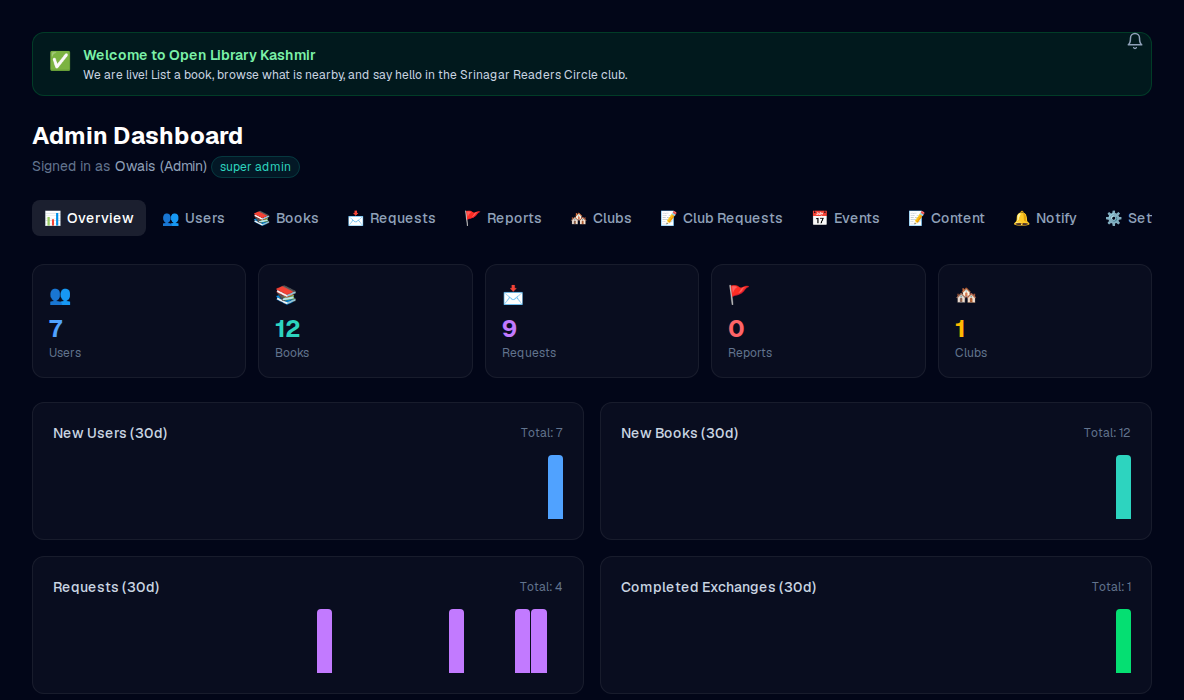
\includegraphics[height=2.5cm]{admin-overview.png}}\hspace{4pt}%
    \fbox{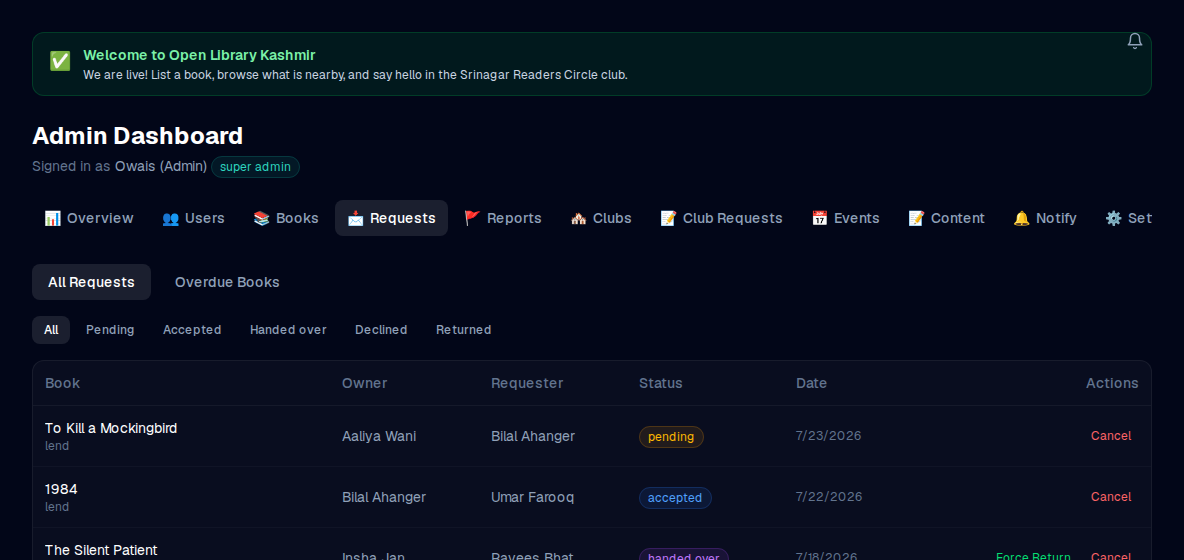
\includegraphics[height=2.5cm]{admin-requests.png}}
  \end{center}
  \vspace{4pt}
  \footnotesize
  \begin{itemize}
    \item Anyone can \textbf{report} a user or a book, any time; moderators triage, ban, warn, or hide in one click.
    \item \textbf{Ten} dedicated admin pages: Overview, Users, Books, Requests (with an Overdue tab), Reports, Clubs, Club Requests, Events, Content, Notifications, Settings.
    \item \textbf{Every} moderation action --- who, what, why, when --- is written to a permanent, tamper-evident audit log that not even a super-admin can edit or delete.
  \end{itemize}
\end{frame}

% ============================================================================
\section{Tech Stack at a Glance}

\begin{frame}{The stack, top to bottom}
  \begin{center}
  \footnotesize
  \begin{tabular}{@{}p{2.6cm}p{3.6cm}p{5.6cm}@{}}
    \toprule
    \textbf{Layer} & \textbf{Technology} & \textbf{Role} \\
    \midrule
    Hosting & Vercel & Builds \& serves the app; runs the weekly digest cron \\
    Framework & Next.js 16 (App Router) & Routing, Server Components, Server Actions \\
    UI runtime & React 19 & Server/Client component model \\
    Language & TypeScript (strict) & All application code \\
    Styling & Tailwind CSS v4 & Utility classes, no component library \\
    Backend & Supabase & Postgres, Auth, REST API, Realtime, Storage \\
    Local dev & Docker (via Supabase CLI) & The same images that could run self-hosted \\
    Email & Resend & Transactional email \& weekly digest \\
    \bottomrule
  \end{tabular}
  \end{center}
\end{frame}

\begin{frame}{Deliberately small, on purpose}
  \begin{itemize}
    \item \textbf{No ORM} --- no Prisma, no Drizzle. Every query goes through Supabase's query builder or a raw Postgres function call.
    \item \textbf{No component library} --- no MUI, Chakra, shadcn. Every button, card, and modal is hand-built.
    \item \textbf{No state-management library}, no React Query/SWR.
  \end{itemize}
  \vfill
  \begin{block}{Why}
    This is a scope choice, not an oversight: keeping the dependency surface small enough that a couple of interns can hold the \emph{entire} system in their heads.
  \end{block}
\end{frame}

\begin{frame}{This codebase pays down its own debt}
  Recent code-quality passes split some of the largest pages in the frontend into hooks and components once they'd grown past a few hundred lines:
  \begin{itemize}
    \item \pathname{my-books/page.tsx}: 905 lines $\to$ a 75-line orchestrator plus five focused components.
    \item \pathname{requests/page.tsx}: 522 lines $\to$ 183, with all fetch/mutation logic moved into a \code{useRequests()} hook.
    \item \pathname{browse/page.tsx}: 683 lines $\to$ 336, with the filter bar and book card promoted to their own components.
  \end{itemize}
  \vfill
  \begin{alertblock}{Why this belongs in an inspiring slide, not just a changelog}
    Nobody made these pages this large on purpose, and nobody was forced to fix them either. Refactoring code that already works, on a deadline-free schedule, is the clearest signal this project cares about the people who'll read this code next --- possibly you.
  \end{alertblock}
\end{frame}

\begin{frame}{Open source, top to bottom}
  \begin{itemize}
    \item Next.js, React, Postgres, PostgREST, GoTrue (auth), Realtime, Storage --- \textbf{every one} of these is open source and self-hostable.
    \item The only pieces that aren't: Vercel's hosting and Resend's email delivery --- both are replaceable, swappable services sitting on top of an otherwise fully open stack.
  \end{itemize}
  \vfill
  \begin{alertblock}{Why this is the whole ballgame for the road-ahead section}
    Because Supabase itself is open source, ``run our own server in Kashmir'' is a realistic plan, not a fantasy --- the exact containers running on a developer's laptop today are what would run on that server.
  \end{alertblock}
\end{frame}

\begin{frame}{A warning for every new contributor}
  \begin{center}
    \Large\textbf{``This is NOT the Next.js you know.''}
  \end{center}
  \vspace{6pt}
  \begin{itemize}
    \item Next.js 16 has real, breaking changes vs.\ most tutorials and training data.
    \item Concrete example: \emph{Middleware} was renamed to \emph{Proxy} --- this project uses \code{src/proxy.ts}, not \code{middleware.ts}.
    \item The project's own \code{AGENTS.md} tells every contributor (human or AI) to check \code{node\_modules/next/dist/docs/} before writing framework-adjacent code.
  \end{itemize}
\end{frame}

% ============================================================================
\section{Under the Hood}

\begin{frame}{System architecture}
  \begin{center}
  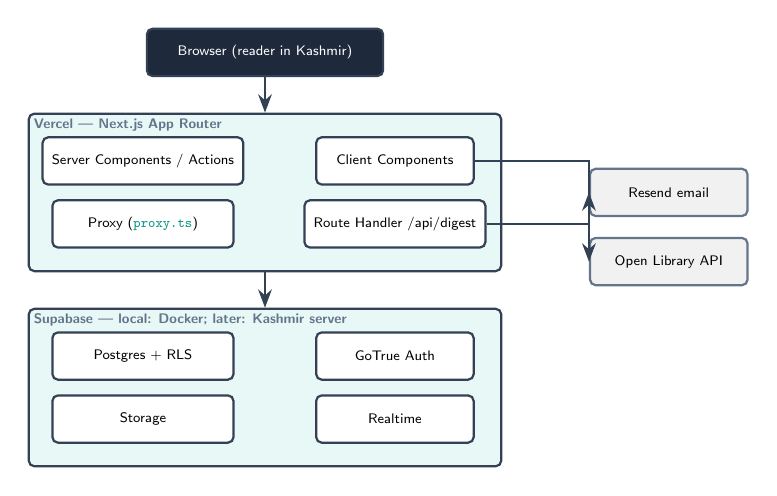
\begin{tikzpicture}[
    box/.style={draw=olkSlateMuted, thick, rounded corners=2pt, minimum height=0.6cm, minimum width=2.3cm, align=center, font=\sffamily\tiny},
    svc/.style={draw=olkSlateMuted, thick, rounded corners=2pt, fill=olkTeal!10},
    ext/.style={box, fill=olkSlate!6, draw=olkGray},
    lbl/.style={font=\sffamily\tiny\bfseries, text=olkGray, anchor=north west, inner sep=2pt},
    arr/.style={-Stealth, thick, olkSlateMuted}
  ]
    \node[box, fill=olkSlateLight, text=white, minimum width=3cm] (browser) {Browser (reader in Kashmir)};
    \node[svc, minimum width=6cm, minimum height=2cm, below=0.45cm of browser] (vercel) {};
    \node[lbl] at (vercel.north west) {Vercel --- Next.js App Router};
    \node[box, fill=white] (rsc) at ($(vercel.center)+(-1.55cm,0.4cm)$) {Server Components / Actions};
    \node[box, fill=white, minimum width=2cm] (cc) at ($(vercel.center)+(1.65cm,0.4cm)$) {Client Components};
    \node[box, fill=white] (proxy) at ($(vercel.center)+(-1.55cm,-0.4cm)$) {Proxy (\code{proxy.ts})};
    \node[box, fill=white, minimum width=2cm] (api) at ($(vercel.center)+(1.65cm,-0.4cm)$) {Route Handler /api/digest};
    \node[svc, minimum width=6cm, minimum height=2cm, below=0.45cm of vercel] (supabase) {};
    \node[lbl] at (supabase.north west) {Supabase --- local: Docker; later: Kashmir server};
    \node[box, fill=white] (pg) at ($(supabase.center)+(-1.55cm,0.4cm)$) {Postgres + RLS};
    \node[box, fill=white, minimum width=2cm] (auth) at ($(supabase.center)+(1.65cm,0.4cm)$) {GoTrue Auth};
    \node[box, fill=white] (storage) at ($(supabase.center)+(-1.55cm,-0.4cm)$) {Storage};
    \node[box, fill=white, minimum width=2cm] (rt) at ($(supabase.center)+(1.65cm,-0.4cm)$) {Realtime};
    \node[ext, right=1.1cm of vercel, minimum width=2cm] (resend) {Resend email};
    \node[ext, below=0.25cm of resend, minimum width=2cm] (olib) {Open Library API};
    \draw[arr] (browser) -- (vercel.north);
    \draw[arr] (vercel) -- (supabase);
    \draw[arr] (api.east) -| (resend.west);
    \draw[arr] (cc.east) -| (olib.west);
  \end{tikzpicture}
  \end{center}
  \small The database box is Docker on a laptop today, and Supabase's hosted cloud in production --- the long-term goal is for that same box to be physical hardware in Kashmir.
\end{frame}

\begin{frame}{Server Components vs.\ Client Components}
  Every file under \code{src/app} is a \textbf{Server Component} unless its first line says \code{"use client"}.
  \begin{itemize}
    \item \textbf{Server}: renders on Vercel, talks to Postgres directly, ships \emph{no} data-fetching code to the browser --- the landing page and every layout.
    \item \textbf{Client}: hydrates and re-renders in the browser, talks to Supabase directly over HTTPS --- subject to Row-Level Security \emph{as the logged-in user}, never an elevated role. Nearly every interactive dashboard page.
  \end{itemize}
  \vfill
  \begin{alertblock}{An honest characteristic, not a recommendation}
    Most of this app's complex pages are Client Components today, even where a Server Component would be more efficient. That's a real, legitimate refactor to propose --- not a rule someone already decided against.
  \end{alertblock}
\end{frame}

\begin{frame}[fragile]{The Proxy layer --- one file, five jobs}
  \code{src/proxy.ts} runs on \emph{every} request, before any page renders:
  \begin{enumerate}
    \item Refresh auth session cookies (unconditional, every request)
    \item Read feature flags from \code{platform\_settings} (cached 30s)
    \item Redirect everyone but admins to \code{/maintenance} when maintenance mode is on
    \item Redirect away from a disabled feature's whole route tree (clubs/wishlists/messages/events)
    \item Gate unauthenticated, banned, and non-admin users off protected routes
  \end{enumerate}
  \vfill
  \small This is the platform-wide switchboard behind the ``one switch, whole platform'' feature-flag slide from the tour.
\end{frame}

\begin{frame}{Supabase fundamentals}
  ``Supabase'' is not one server --- it's a bundle of independent, cooperating open-source services in front of stock Postgres:
  \begin{itemize}
    \item \textbf{Postgres} --- the real database; every table is a plain, non-proprietary table.
    \item \textbf{PostgREST} --- turns the schema into a REST API automatically. No hand-written backend for most operations.
    \item \textbf{GoTrue} --- issues/verifies JWTs, owns \code{auth.users}.
    \item \textbf{Storage} --- S3-like object store (book cover images).
    \item \textbf{Realtime} --- streams row changes over WebSockets --- powers chat and the notification bell.
  \end{itemize}
\end{frame}

\begin{frame}{The database, at a glance}
  \textbf{27 tables}, all in \code{public}, every one Row-Level-Security protected.
  \footnotesize
  \begin{columns}[T]
    \column{0.5\textwidth}
    \textbf{Identity \& exchange}
    \begin{itemize}
      \item \code{profiles}, \code{books}
      \item \code{book\_requests}, \code{book\_progress}
    \end{itemize}
    \textbf{Community}
    \begin{itemize}
      \item \code{messages}, \code{wishlists}, \code{ratings}
      \item \code{bookmarks}, \code{book\_notes}
    \end{itemize}
    \textbf{Clubs \& events}
    \begin{itemize}
      \item \code{clubs} (+members, posts, requests)
      \item \code{club\_events}, \code{event\_rsvps}
    \end{itemize}
    \column{0.5\textwidth}
    \textbf{Notifications \& content}
    \begin{itemize}
      \item \code{notifications} (+templates)
      \item \code{announcements}, \code{genres}, \code{areas}
      \item \code{book\_of\_month}, \code{platform\_settings}
    \end{itemize}
    \textbf{Admin \& moderation}
    \begin{itemize}
      \item \code{reports}, \code{user\_bans/warnings}
      \item \code{admin\_audit\_log}, \code{admin\_notes}
    \end{itemize}
  \end{columns}
  \vfill
  \normalsize\textbf{No ORM} --- the schema itself, not generated code, is the single source of truth.
\end{frame}

\begin{frame}{\code{auth.users} vs.\ \code{public.profiles}}
  \begin{itemize}
    \item Supabase Auth owns \code{auth.users} --- email, password hash. Application code never touches it directly.
    \item \code{public.profiles} mirrors what the app actually needs (name, area, admin role, ban state).
    \item Kept in lock-step by \textbf{one database trigger}, fired the instant someone signs up.
  \end{itemize}
  \vfill
  \begin{alertblock}{A real, consequential exception}
    \code{books.owner\_id} points at \code{auth.users}, not \code{profiles} --- so fetching ``the book owner's name'' always needs a second, separate query. This is documented \emph{in the code itself} as the single best piece of institutional memory in the whole frontend.
  \end{alertblock}
\end{frame}

\begin{frame}{Row-Level Security --- the real security model}
  \begin{itemize}
    \item Every table: RLS \textbf{enabled}, default \textbf{closed}. No matching policy means no rows --- for anyone, through any route.
    \item Postgres checks every query against \code{auth.uid()} / \code{auth.role()} from the caller's own JWT.
    \item For ordinary data access, \textbf{there is no separate authorization layer} in the application --- the database \emph{is} the security boundary.
  \end{itemize}
  \vfill
  \begin{block}{Three admin roles, one hierarchy}
    \code{viewer} $\prec$ \code{moderator} $\prec$ \code{super\_admin} --- checked in exactly one place (\code{is\_admin\_or\_mod()}, \code{is\_super\_admin()}), not duplicated across every policy that needs it.
  \end{block}
\end{frame}

\begin{frame}[fragile]{\code{SECURITY DEFINER}: the escape hatch, used carefully}
  Some features \emph{need} to cross the RLS boundary on purpose: matching your wishlist against a book someone else just listed means searching \emph{everyone's} wishlist rows, not just your own.
  \begin{itemize}
    \item Solution: a narrow Postgres function that runs with elevated privilege --- but only returns exactly the columns it was written to return.
    \item Discipline enforced throughout: never \code{SELECT *} on a sensitive table; explicit \code{REVOKE}/\code{GRANT} on the risky ones.
  \end{itemize}
  \vfill
  \begin{alertblock}{Why this matters}
    A bug in one of these functions is a bug that runs with elevated privilege --- it is exactly as dangerous as it is useful.
  \end{alertblock}
\end{frame}

\begin{frame}[fragile]{How location actually works}
  \begin{itemize}
    \item No PostGIS, no Google Maps API. Just two floats --- \code{latitude}/\code{longitude} --- on \code{profiles}, \code{clubs}, and now \code{club\_events}, captured via the browser's native \code{navigator.geolocation} API.
    \item \code{area\_name} is a free-text label shown \emph{alongside} the coordinates --- approximate, human, never an exact street address.
  \end{itemize}
  \begin{lstlisting}
6371 * acos( cos(lat1)*cos(lat2)*cos(lng2-lng1)
             + sin(lat1)*sin(lat2) )   -- distance, in km
  \end{lstlisting}
  \small That's the entire ``nearby'' feature: the haversine great-circle formula, running as one Postgres function, sorting results by real distance. A clamp (\code{LEAST}/\code{GREATEST}) guards against a floating-point edge case that once made this return \code{NaN} for a user browsing their own listing.
\end{frame}

\begin{frame}{Defense in depth: rate limiting \& validation}
  Every important limit lives in the \textbf{database}, not just the UI --- so it holds even against a direct API call:
  \begin{itemize}
    \item Max messages/hour and requests/day --- enforced by \code{BEFORE INSERT} triggers, reading their limits from \code{platform\_settings}.
    \item Club-creation eligibility (5+ completed exchanges, no reports) and event RSVP capacity --- both checked client-side \emph{and} re-checked by a database trigger or policy.
    \item Free-text search is sanitised before being interpolated into the query filter DSL --- the same category of defence as SQL parameterisation.
  \end{itemize}
\end{frame}

\begin{frame}{Docker \& local development}
  \begin{itemize}
    \item The \emph{entire} Supabase stack --- Postgres, GoTrue, PostgREST, Realtime, Storage, Studio --- runs as Docker containers via the Supabase CLI. One command: \code{npx supabase start}.
    \item 32 migrations, replayed from scratch with \code{supabase db reset} any time local state is in doubt.
    \item Local and production are deliberately structured to be near-identical: same migrations, same RLS policies, same functions.
  \end{itemize}
  \vfill
  \begin{alertblock}{Not just developer convenience}
    Every hour spent comfortable with this Docker stack is rehearsal for the day it runs on real hardware in Kashmir instead of a laptop.
  \end{alertblock}
\end{frame}

\begin{frame}{Deployment, today}
  \begin{itemize}
    \item \textbf{Vercel} builds and serves the frontend --- push to the connected branch, it redeploys automatically; PRs get their own preview.
    \item \textbf{Database migrations} are pushed separately: \code{supabase db push} against the hosted project --- forward-only, no reset-and-replay safety net in production.
    \item The \textbf{weekly digest} is a real cron-triggered endpoint, authenticated with a shared secret, sending in batches --- built to survive well past today's user count.
  \end{itemize}
  \vfill
  \small The service-role key that bypasses RLS entirely never reaches the browser --- enforced at \emph{build time}, not just by convention.
\end{frame}

\begin{frame}{Honest accounting: what's still open}
  \begin{itemize}
    \item Automated test coverage is minimal --- a handful of unit tests, no end-to-end coverage yet.
    \item No production error monitoring --- no Sentry, no Vercel Analytics; a runtime error today is invisible unless a user reports it.
    \item No general HTTP-level rate limiting yet --- only two database triggers, scoped to messages and requests.
    \item \code{/browse}'s \code{.limit(200)} is a stopgap, not real pagination --- fine for now, a real fix is already scoped.
    \item Admin list pages other than Books have no pagination yet --- lower priority, since admin traffic is small.
  \end{itemize}
  \vfill
  \begin{block}{This is not a secret}
    All of this --- and the reasoning behind every design decision in this section --- lives in \code{Guide/main.pdf}, kept as the living source of truth, updated the same day a fix ships.
  \end{block}
\end{frame}

% ============================================================================
\section{The Road Ahead}

\begin{frame}{A mobile app, on the same backend}
  \begin{itemize}
    \item Supabase's API is transport-agnostic --- a React Native / Expo (or Flutter) app talks to the \emph{exact same} Postgres, the same RLS policies, the same auth. No separate backend to build.
    \item Push notifications would sit naturally alongside --- or eventually replace --- the email digest.
    \item Worth designing for from day one: offline-first behaviour for areas with patchy connectivity.
  \end{itemize}
\end{frame}

\begin{frame}{Two real infrastructure audits, and what we learned}
  In July 2026, an external review proposed a full self-hosting migration --- VPS, self-hosted Supabase, self-hosted mail --- sized for \textbf{100,000} users.
  \vspace{4pt}
  \begin{alertblock}{The lesson, stated plainly}
    The individual pieces were technically sound. The problem was the framing: \textbf{the 100k figure had no basis} --- this project was pre-launch at the time. Self-hosted email on a fresh server would likely land in spam, defeating the point. The decision: stay on Vercel + managed Supabase + Resend until there's real load to justify the move.
  \end{alertblock}
  A second, narrower audit two weeks later asked a better question --- ``is this ready to go live, and does it survive real growth?'' --- and found concrete bugs (missing indexes, an unbounded query, an N+1 in the digest cron), all fixed the same day.
  \vfill
  \small This is the habit worth taking away: solve the problem you can prove you have, not the one that sounds impressive.
\end{frame}

\begin{frame}{The scaling roadmap, phase by phase}
  \begin{center}
  \footnotesize
  \begin{tabular}{@{}p{1.6cm}p{3.0cm}p{7.6cm}@{}}
    \toprule
    \textbf{Phase} & \textbf{Starts when...} & \textbf{What changes} \\
    \midrule
    0 --- Done & --- & Indexes, bounded queries, batched digest, deduped auth, one small cache. \\
    1 --- Harden & Now, toward 30--50k users & Real pagination, general rate limiting, error monitoring, a proper geo-query fix, plan upgrades. \\
    2 --- Rehearse & 2+ developers, Phase 1 stable & Run the already-Dockerised Supabase stack on a rented VPS, in parallel with production. \\
    3 --- Sovereignty & VPS rehearsal proven over months & Move the same, already-proven stack onto physical hardware in Kashmir. \\
    \bottomrule
  \end{tabular}
  \end{center}
  \vfill
  \begin{alertblock}{The rule that governs every row above}
    Don't start a phase before its trigger condition is actually true --- the same discipline the 100k lesson taught, applied forward instead of in hindsight.
  \end{alertblock}
\end{frame}

\begin{frame}{Why self-hosting is worth the long game}
  \begin{itemize}
    \item Every Supabase service is open source and self-hostable --- nothing about today's architecture is a rented black box.
    \item The Docker stack developers already run daily \emph{is} the rehearsal for a physical server in-region.
    \item Why it matters: less dependency on foreign-hosted infrastructure, data sovereignty over community members' information, and long-term cost control.
  \end{itemize}
  \vfill
  \begin{block}{A VPS alone is not the goal}
    Renting a generic VPS just swaps one third party's control for another's. It only counts as progress if it's treated as a rehearsal for physical hardware --- Phase 2 above, not a destination in itself.
  \end{block}
\end{frame}

\begin{frame}{More creative ideas, worth a conversation}
  \begin{itemize}
    \item SMS/WhatsApp notifications for areas with limited smartphone data plans.
    \item Partnerships with schools and libraries --- bulk onboarding, organised ``book drive'' events (Book-of-the-Month, Announcements, and now Events already exist to support campaigns like this).
    \item Multi-language UI --- Kashmiri, Urdu, English.
    \item A public, read-only stats page --- transparency about community impact.
    \item Community-run local ``book hubs'': a reading club paired with a physical drop-off point.
  \end{itemize}
\end{frame}

% ============================================================================
\section{Get Involved}

\begin{frame}{Two ways to help, starting today}
  \begin{columns}[T]
    \column{0.48\textwidth}
    \textbf{If you're a developer}
    \begin{itemize}
      \item Run it locally: \code{npx supabase start \&\& npm run dev}
      \item Read the chapter behind anything in this deck --- \code{Guide/main.pdf}
      \item Pick one item from Phase 1 of the roadmap and send a PR
    \end{itemize}
    \column{0.48\textwidth}
    \textbf{If you're a first-phase user}
    \begin{itemize}
      \item List your first book --- lend or donate, scanner does the rest
      \item Browse what's nearby and send your first request
      \item Tell us what's confusing --- your feedback \emph{is} the roadmap
    \end{itemize}
  \end{columns}
  \vfill
  \begin{alertblock}{Why your feedback matters more than usual, right now}
    This platform exists because a volunteer-run model couldn't reach enough people. You are the test of whether the replacement actually works --- not a beta tester of a finished product, but a co-author of what it becomes next.
  \end{alertblock}
\end{frame}

\begin{frame}{Thank you --- let's get involved}
  \begin{itemize}
    \item \textbf{Start here:} \code{Guide/main.pdf} --- the full technical manual, written specifically for new maintainers.
    \item \textbf{Run it locally:} \code{npx supabase start \&\& npm run dev}.
    \item Every design decision in this deck has a chapter, a migration, or a line of code behind it --- nothing here was hand-waved, and nothing you saw on screen was staged.
  \end{itemize}
  \vfill
  \begin{center}
    \Large\textbf{Questions \& discussion}
  \end{center}
\end{frame}

\end{document}
